% ==========================================
% GRAFICI E TABELLE CAPITOLO 5
% ==========================================
% Nota: Aggiungere nel preambolo:
\documentclass{article}
\usepackage{pgfplots}
\usepackage{tikz}
\usetikzlibrary{shapes,arrows,positioning,calc,patterns,decorations.pathreplacing}
\usepackage{booktabs}
\usepackage{array}
\usepackage{multirow}
\pgfplotsset{compat=1.18}
\usetikzlibrary{shapes,arrows,positioning,calc,patterns,decorations.pathreplacing}
\usepackage{multirow}
\usepackage{amsmath}    
\usepackage{amssymb}
\usepackage{pgfplotstable}
\usepackage{graphicx}

\usepackage{geometry}
\geometry{a4paper, margin=1in}  




% ==========================================
% FIGURA 5.1: Framework GIST - Modello Integrato
% ==========================================
\begin{document}
%\resizebox{\textwidth}{!}{...} % per la tabella larga


\begin{figure}[htbp]
\centering
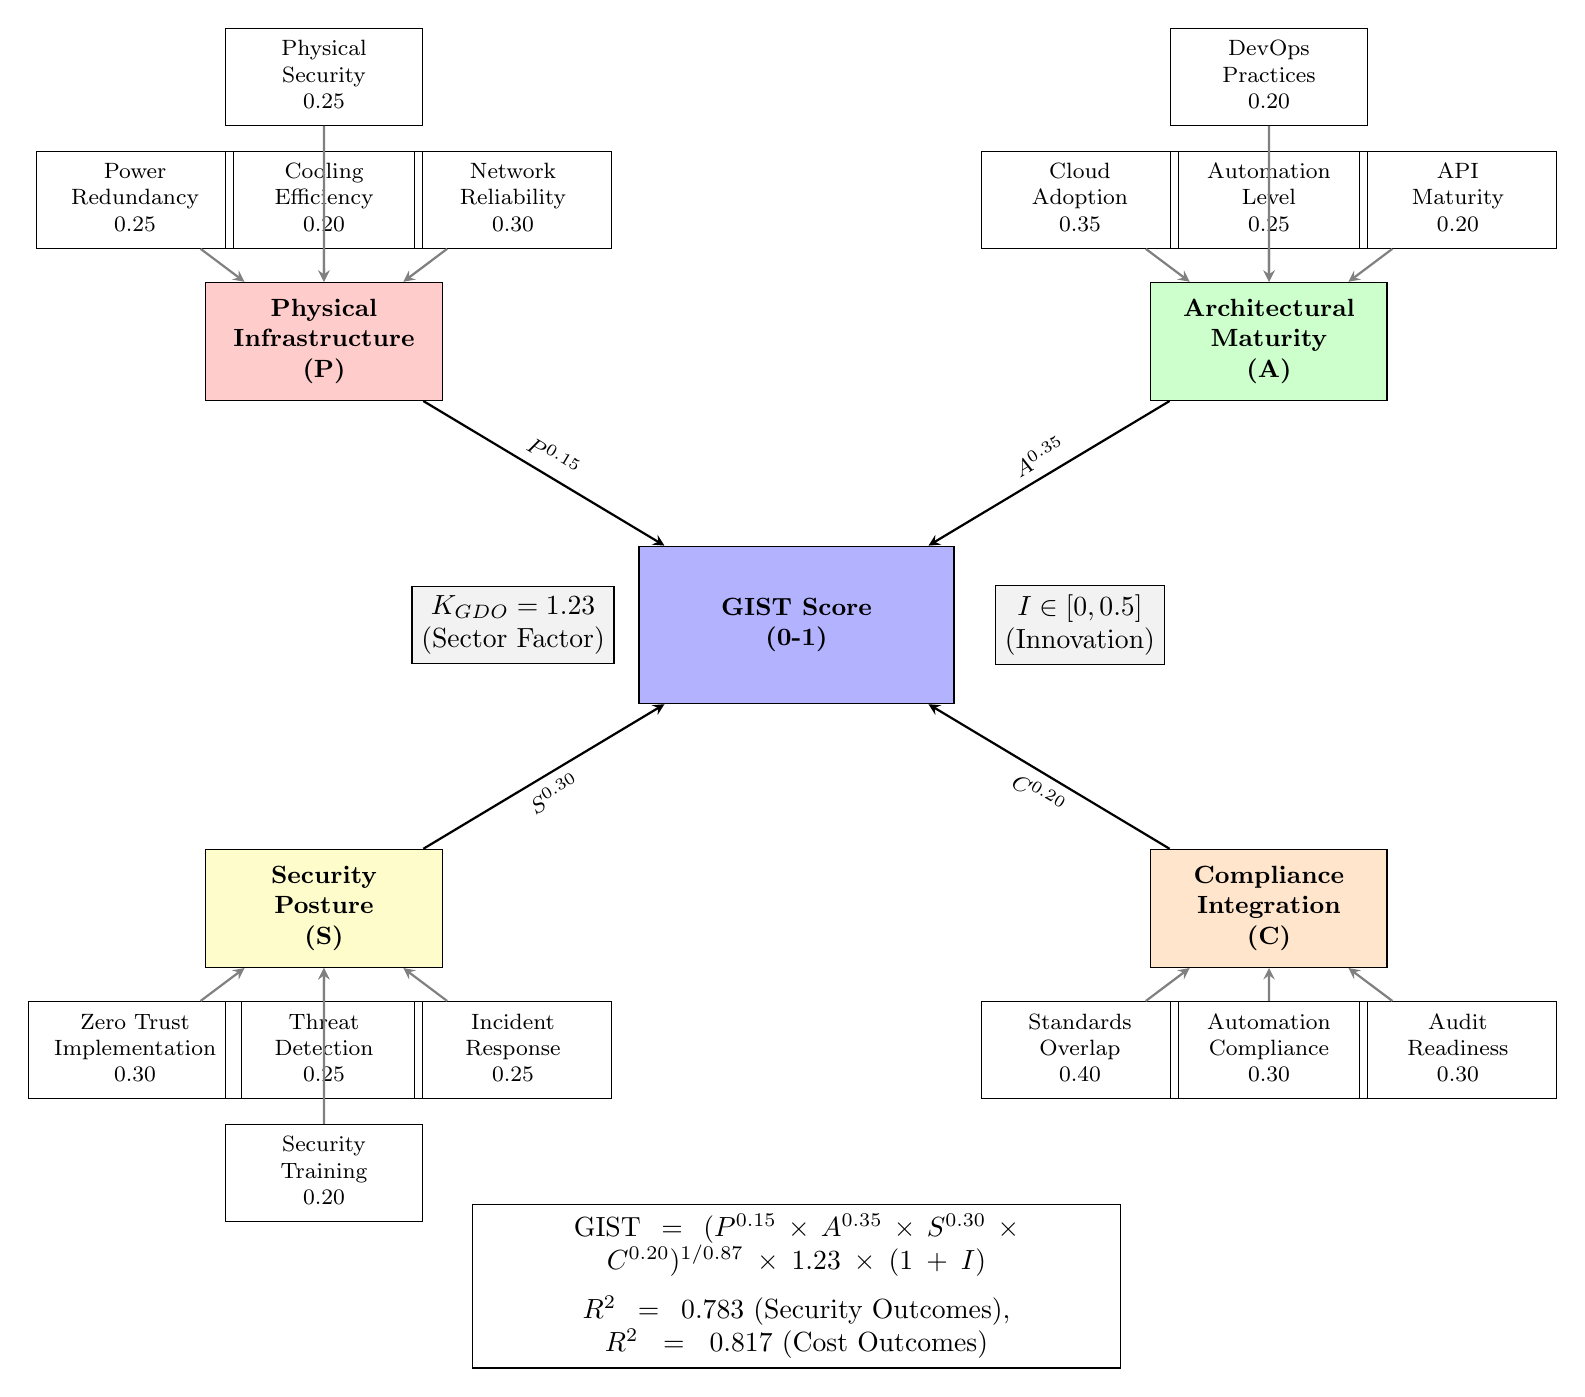
\begin{tikzpicture}[scale=1.2]
    % Stili
    \tikzset{
        component/.style={rectangle, draw, minimum width=3cm, minimum height=1.5cm, text centered, font=\small\bfseries},
        subcomp/.style={rectangle, draw, minimum width=2.5cm, minimum height=0.8cm, text centered, font=\footnotesize},
        arrow/.style={->, thick, >=stealth},
        coefficient/.style={font=\footnotesize\itshape}
    }
    
    % Componente centrale GIST
    \node[component, fill=blue!30, minimum width=4cm, minimum height=2cm, align=center] (gist) at (0,0) {GIST Score\\(0-1)};
    
    % Componenti principali
    \node[component, fill=red!20,align=center] (physical) at (-5,3) {Physical\\Infrastructure\\(P)};
    \node[component, fill=green!20,align=center] (arch) at (5,3) {Architectural\\Maturity\\(A)};
    \node[component, fill=yellow!20,align=center] (security) at (-5,-3) {Security\\Posture\\(S)};
    \node[component, fill=orange!20,align=center] (compliance) at (5,-3) {Compliance\\Integration\\(C)};
    
    % Subcomponenti Physical
    \node[subcomp] (p1) at (-7,4.5) {\begin{tabular}{c}Power\\Redundancy\\0.25\end{tabular}};
    \node[subcomp] (p2) at (-5,4.5) {\begin{tabular}{c}Cooling\\Efficiency\\0.20\end{tabular}};
    \node[subcomp] (p3) at (-3,4.5) {\begin{tabular}{c}Network\\Reliability\\0.30\end{tabular}};
    \node[subcomp] (p4) at (-5,5.8) {\begin{tabular}{c}Physical\\Security\\0.25\end{tabular}};
    
    % Subcomponenti Architecture
    \node[subcomp] (a1) at (3,4.5) {\begin{tabular}{c}Cloud\\Adoption\\0.35\end{tabular}};
    \node[subcomp] (a2) at (5,4.5) {\begin{tabular}{c}Automation\\Level\\0.25\end{tabular}};
    \node[subcomp] (a3) at (7,4.5) {\begin{tabular}{c}API\\Maturity\\0.20\end{tabular}};
    \node[subcomp] (a4) at (5,5.8) {\begin{tabular}{c}DevOps\\Practices\\0.20\end{tabular}};
    
    % Subcomponenti Security
    \node[subcomp] (s1) at (-7,-4.5) {\begin{tabular}{c}Zero Trust\\Implementation\\0.30\end{tabular}};
    \node[subcomp] (s2) at (-5,-4.5) {\begin{tabular}{c}Threat\\Detection\\0.25\end{tabular}};
    \node[subcomp] (s3) at (-3,-4.5) {\begin{tabular}{c}Incident\\Response\\0.25\end{tabular}};
    \node[subcomp] (s4) at (-5,-5.8) {\begin{tabular}{c}Security\\Training\\0.20\end{tabular}};
    
    % Subcomponenti Compliance
    \node[subcomp] (c1) at (3,-4.5) {\begin{tabular}{c}Standards\\Overlap\\0.40\end{tabular}};
    \node[subcomp] (c2) at (5,-4.5) {\begin{tabular}{c}Automation\\Compliance\\0.30\end{tabular}};
    \node[subcomp] (c3) at (7,-4.5) {\begin{tabular}{c}Audit\\Readiness\\0.30\end{tabular}};
    
    % Frecce dai subcomponenti ai componenti
    \foreach \i in {1,2,3,4} {
        \draw[arrow, gray] (p\i) -- (physical);
        \draw[arrow, gray] (a\i) -- (arch);
        \draw[arrow, gray] (s\i) -- (security);
    }
    \foreach \i in {1,2,3} {
        \draw[arrow, gray] (c\i) -- (compliance);
    }
    
    % Frecce dai componenti a GIST con coefficienti
    \draw[arrow] (physical) -- node[coefficient, above, sloped] {$P^{0.15}$} (gist);
    \draw[arrow] (arch) -- node[coefficient, above, sloped] {$A^{0.35}$} (gist);
    \draw[arrow] (security) -- node[coefficient, below, sloped] {$S^{0.30}$} (gist);
    \draw[arrow] (compliance) -- node[coefficient, below, sloped] {$C^{0.20}$} (gist);
    
    % Formula completa
    \node[draw, fill=white, text width=8cm, align=center] at (0,-7) {
        $\text{GIST} = (P^{0.15} \times A^{0.35} \times S^{0.30} \times C^{0.20})^{1/0.87} \times 1.23 \times (1 + I)$\\
        \vspace{0.2cm}
        $R^2 = 0.783$ (Security Outcomes), $R^2 = 0.817$ (Cost Outcomes)
    };
    
    % Fattori moltiplicativi
    \node[draw, fill=gray!10,align=center] at (-3,0) {$K_{GDO} = 1.23$\\(Sector Factor)};
    \node[draw, fill=gray!10,align=center] at (3,0) {$I \in [0, 0.5]$\\(Innovation)};
    
\end{tikzpicture}
\caption{Framework GIST - Modello Integrato con Coefficienti Validati Empiricamente}
\label{fig:gist-framework}
\end{figure}

% ==========================================
% TABELLA 5.1: Roadmap Implementativa
% ==========================================

\begin{table}[htbp]
\centering
\caption{Roadmap Implementativa GIST - Metriche e Dipendenze per Wave}
\label{tab:roadmap-gist}
\resizebox{\textwidth}{!}{%
\begin{tabular}{@{}lcccccccc@{}}
\toprule
\textbf{Wave/Intervento} & \textbf{Priority} & \textbf{Costo} & \textbf{ROI} & \textbf{Impatto} & \textbf{Riduzione} & \textbf{Dipendenze} & \textbf{Risorse} & \textbf{Timeline} \\
 & \textbf{Score} & \textbf{(€K)} & \textbf{(mesi)} & \textbf{GIST} & \textbf{Rischio} & & \textbf{FTE} & \textbf{(mesi)} \\
\midrule
\multicolumn{9}{l}{\textbf{Wave 1: Quick Wins (0-6 mesi)}} \\
\midrule
MFA Estesa & 8.7 & 125 & 4 & +0.08 & 31\% & Nessuna & 2.5 & 2 \\
Network Segmentation Base & 8.2 & 340 & 7 & +0.12 & 24\% & MFA & 4.0 & 3 \\
Compliance Mapping & 7.9 & 85 & 3 & +0.05 & 43\%$^*$ & Nessuna & 1.5 & 2 \\
\textbf{Subtotale Wave 1} & & \textbf{550} & \textbf{5} & \textbf{+0.25} & & & \textbf{8.0} & \textbf{6} \\
\midrule
\multicolumn{9}{l}{\textbf{Wave 2: Core Transformation (6-18 mesi)}} \\
\midrule
SD-WAN Complete & 7.6 & 1,200 & 14 & +0.15 & 47\%$^{**}$ & Segmentation & 6.0 & 6 \\
Cloud Migration Selective & 7.3 & 2,800 & 19 & +0.18 & 23\%$^{***}$ & SD-WAN & 8.0 & 8 \\
Zero Trust Phase 1 & 7.1 & 1,700 & 16 & +0.20 & 28\% & Cloud Base & 5.0 & 6 \\
\textbf{Subtotale Wave 2} & & \textbf{5,700} & \textbf{17} & \textbf{+0.53} & & & \textbf{19.0} & \textbf{12} \\
\midrule
\multicolumn{9}{l}{\textbf{Wave 3: Advanced Optimization (18-36 mesi)}} \\
\midrule
AI Security Operations & 6.8 & 2,300 & 24 & +0.12 & 67\%$^{\dagger}$ & Zero Trust & 4.0 & 9 \\
Full Cloud Transform & 6.4 & 5,700 & 28 & +0.15 & 38\%$^{\dagger\dagger}$ & Cloud Select & 10.0 & 12 \\
Autonomous Compliance & 6.1 & 1,100 & 21 & +0.08 & 39\%$^{\dagger\dagger\dagger}$ & AI Ops & 3.0 & 6 \\
\textbf{Subtotale Wave 3} & & \textbf{9,100} & \textbf{26} & \textbf{+0.35} & & & \textbf{17.0} & \textbf{18} \\
\midrule
\textbf{TOTALE} & & \textbf{15,350} & \textbf{22} & \textbf{+1.13} & & & \textbf{44.0} & \textbf{36} \\
\bottomrule
\end{tabular}%
}
\vspace{0.3cm}
\footnotesize
\begin{flushleft}
$^*$Efficienza audit | $^{**}$Availability improvement | $^{***}$TCO reduction | $^{\dagger}$MTTR reduction | $^{\dagger\dagger}$TCO total | $^{\dagger\dagger\dagger}$Compliance cost
\end{flushleft}
\end{table}

% ==========================================
% FIGURA 5.2: Matrice Impatto-Probabilità
% ==========================================
\begin{figure}[htbp]
\centering
\begin{tikzpicture}
\begin{axis}[
    width=0.85\textwidth,
    height=0.7\textwidth,
    xlabel={Probabilità di Realizzazione (\%)},
    ylabel={Impatto sul Business (1-10)},
    xmin=0, xmax=100,
    ymin=0, ymax=10,
    grid=major,
    grid style={line width=.1pt, draw=gray!30},
    ]
    
    % Quadranti colorati
    \fill[green!10] (axis cs:0,0) rectangle (axis cs:50,5);
    \fill[yellow!10] (axis cs:50,0) rectangle (axis cs:100,5);
    \fill[yellow!10] (axis cs:0,5) rectangle (axis cs:50,10);
    \fill[red!10] (axis cs:50,5) rectangle (axis cs:100,10);
    
    % Labels quadranti
    \node[anchor=center] at (axis cs:25,2.5) {\textbf{Monitor}};
    \node[anchor=center] at (axis cs:75,2.5) {\textbf{Prepare}};
    \node[anchor=center] at (axis cs:25,7.5) {\textbf{Ricerca}};
    \node[anchor=center] at (axis cs:75,7.5) {\textbf{Act Now}};
    
    % Trend points con labels
    \node[mark=*, mark size=4pt, color=blue] (quantum) at (axis cs:73,8.5) {};
    \node[anchor=west, font=\small] at (quantum) {Quantum Computing};
    
    \node[mark=*, mark size=4pt, color=blue] (ai) at (axis cs:85,7.2) {};
    \node[anchor=west, font=\small] at (ai) {AI Generativa};
    
    \node[mark=*, mark size=4pt, color=blue] (sixg) at (axis cs:45,7.8) {};
    \node[anchor=east, font=\small] at (sixg) {6G Networks};
    
    \node[mark=*, mark size=4pt, color=blue] (blockchain) at (axis cs:67,5.5) {};
    \node[anchor=south, font=\small] at (blockchain) {Blockchain SC};
    
    \node[mark=*, mark size=4pt, color=blue] (aiact) at (axis cs:95,6.8) {};
    \node[anchor=west, font=\small] at (aiact) {AI Act};
    
    \node[mark=*, mark size=4pt, color=blue] (cra) at (axis cs:92,7.5) {};
    \node[anchor=south, font=\small] at (cra) {Cyber Resilience Act};
    
    \node[mark=*, mark size=4pt, color=blue] (gdpr2) at (axis cs:78,6.2) {};
    \node[anchor=south, font=\small] at (gdpr2) {GDPR Evolution};
    
    \node[mark=*, mark size=4pt, color=blue] (green) at (axis cs:88,8.9) {};
    \node[anchor=south, font=\small] at (green) {Green IT Mandates};
    
    % Error bars per uncertainty
    \foreach \point in {quantum,ai,sixg,blockchain,aiact,cra,gdpr2,green} {
        \draw[gray, thick] (axis cs:\point) ++(axis cs:-5,0) -- ++(axis cs:10,0);
        \draw[gray, thick] (axis cs:\point) ++(axis cs:0,-0.3) -- ++(axis cs:0,0.6);
    }
    
    % Timeline indicators
    \draw[thick, dashed, ->] (axis cs:10,9) -- (axis cs:90,9);
    \node[anchor=south] at (axis cs:20,9) {2025};
    \node[anchor=south] at (axis cs:50,9) {2027};
    \node[anchor=south] at (axis cs:80,9) {2030};
  
    % Legenda impatto finanziario
    \node[draw, fill=white, anchor=north east] at (axis cs:98,4) {
    \begin{tabular}{lr}
    \multicolumn{2}{l}{\textbf{Impatto Stimato}}\\
    \hline
    Quantum: & €2.3M\\
    AI Gen: & €0.9M\\
    6G: & €1.5M\\
    Blockchain: & €0.7M\\
    AI Act: & €1.5M\\
    CRA: & €2.4M\\
    GDPR++: & €0.8M\\
    Green IT: & €4.2M\\
    \hline
    \textbf{Totale:} & \textbf{€14.3M}
    \end{tabular}
    };
\end{axis}
\end{tikzpicture}
\caption{Matrice Impatto-Probabilità dei Trend Emergenti 2025-2030}
\label{fig:trend-matrix}
\end{figure}

% ==========================================
% FIGURA 5.3: Vision 2030 - GDO Cyber-Resiliente
% ==========================================

\begin{figure}[htbp]
\centering
\begin{tikzpicture}[scale=0.9]
    % Stili
    \tikzset{
        pillar/.style={rectangle, draw, minimum width=2.5cm, minimum height=4cm, text centered, font=\small\bfseries},
        element/.style={rectangle, draw, minimum width=2.2cm, minimum height=0.6cm, text centered, font=\footnotesize},
        vision/.style={ellipse, draw, minimum width=4cm, minimum height=2cm, text centered, font=\bfseries},
        arrow/.style={->, thick, >=stealth},
        metric/.style={font=\footnotesize\itshape}
    }
    
    % Vision centrale
    \node[vision, fill=blue!30, minimum width=6cm] (vision) at (0,0) {GDO 2030\\Cyber-Resiliente\\GIST Score ≥0.85};
    
    % Pilastri principali
    \node[pillar, fill=green!20] (infra) at (-6,0) {Infrastructure\\4.0};
    \node[pillar, fill=yellow!20] (security) at (-2,0) {Autonomous\\Security};
    \node[pillar, fill=orange!20] (compliance) at (2,0) {Continuous\\Compliance};
    \node[pillar, fill=red!20] (business) at (6,0) {Business\\Innovation};
    
    % Elementi Infrastructure
    \node[element] at (-6,1.5) {100\% Cloud};
    \node[element] at (-6,0.8) {Quantum-Ready};
    \node[element] at (-6,0.1) {Zero Carbon};
    \node[element] at (-6,-0.6) {Self-Healing};
    \node[element] at (-6,-1.3) {6G Connected};
    
    % Elementi Security
    \node[element] at (-2,1.5) {AI-Driven SOC};
    \node[element] at (-2,0.8) {Predictive Defense};
    \node[element] at (-2,0.1) {Zero Trust Native};
    \node[element] at (-2,-0.6) {99.99\% Uptime};
    \node[element] at (-2,-1.3) {<1min MTTR};
    
    % Elementi Compliance
    \node[element] at (2,1.5) {Real-time Audit};
    \node[element] at (2,0.8) {Auto-Remediation};
    \node[element] at (2,0.1) {Multi-Standard};
    \node[element] at (2,-0.6) {Zero Violations};
    \node[element] at (2,-1.3) {90\% Automated};
    
    % Elementi Business
    \node[element] at (6,1.5) {+40\% Revenue};
    \node[element] at (6,0.8) {New Services};
    \node[element] at (6,0.1) {Trust Premium};
    \node[element] at (6,-0.6) {Market Leader};
    \node[element] at (6,-1.3) {ROI 340\%};
    
    % Metriche di transizione
    \node[draw, fill=gray!10, text width=10cm] at (0,-3.5) {
        \textbf{Journey 2024-2030:} GIST 0.45 → 0.85 | Investment €15.4M | ROI 340\% | Risk -89\%
    };
    
    % Timeline arrows
    \draw[arrow, ultra thick, green!50!black] (-8,-4.5) -- node[above] {2024} (-6,-4.5);
    \draw[arrow, ultra thick, yellow!50!black] (-6,-4.5) -- node[above] {2026} (-2,-4.5);
    \draw[arrow, ultra thick, orange!50!black] (-2,-4.5) -- node[above] {2028} (2,-4.5);
    \draw[arrow, ultra thick, red!50!black] (2,-4.5) -- node[above] {2030} (6,-4.5);
    
    % Outcome metrics
    \node[metric] at (-7,-5) {Foundation};
    \node[metric] at (-3,-5) {Transformation};
    \node[metric] at (1,-5) {Optimization};
    \node[metric] at (5,-5) {Leadership};
    
    % Business value equation
    \node[draw, fill=white] at (0,3.5) {
        $\text{Value}_{2030} = \text{Security} + \text{Efficiency} + \text{Innovation} + \text{Trust} = \text{Competitive Advantage}$
    };
    
\end{tikzpicture}
\caption{Vision 2030 - La GDO Cyber-Resiliente del Futuro}
\label{fig:vision-2030}
\end{figure}

\end{document}